
When having to compose concurrent systems we define three different semantics that can be applied pairwise. Synchronous semantic $A ||_s B$ (Figure~\ref{fig:synchronous_composition})captures the composition of two components that share a single synchronizing event (implicit), where all participants should be able to make progress concurrently. The main motivation being digital components sharing a single clock. 
Asynchronous semantic $A ||_a B$ (Figure~\ref{fig:asynchronous_composition}) captures the interleaving interpretation of concurrency as found in LTS systems. 

\begin{figure}[h]
		\centering
	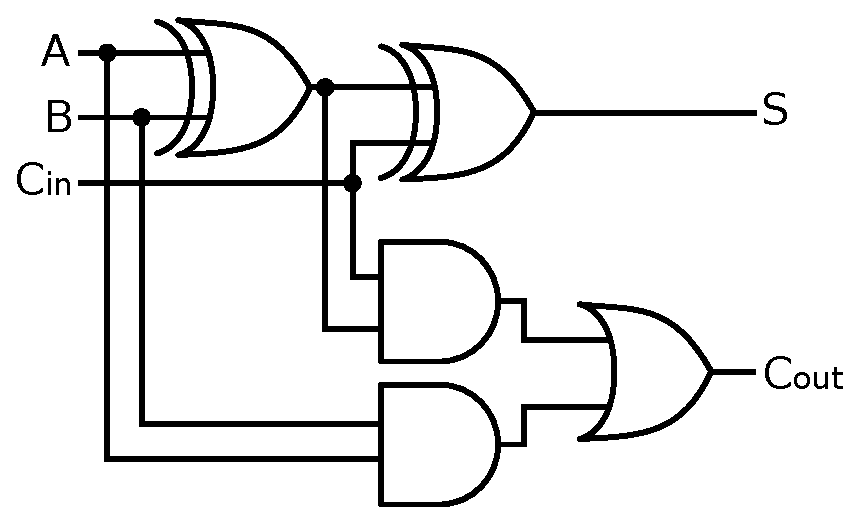
\includegraphics[scale=.4]{img/full-adder.eps}
	\caption{Full adder circuit}
	\label{fig:full_adder_circuit}
\end{figure}

A motivation for the synchronous composition can be found in the following example: a digital design consists of two 1 bit full adders working as separate units. Let $i \in \{1,2\}$ be the index of each adder and $a$ and $b$ the 1 bit entries to be added, $c\_in_i$ the incoming carry signal from another module, $s_i$ the output that represents the lower bit of the sum and $c_i$ the upper bit or carry out, then each 1 bit full adder can be modeled as a single state CLTS.  The FSP syntax would be the following:

\renewcommand{\ttdefault}{pcr}
\begin{figure}[H]
	\begin{lstlisting}[escapeinside={[*}{*]},basicstyle=\scriptsize\ttfamily,columns=flexible,mathescape=true,xleftmargin=3.0ex,keywordstyle=\textbf,morekeywords={if,while,do,else,fork,int,null, algorithm, is, input, output, return, for}]
	FULL_ADDER[i] = (<a[i],s[i]> -> FULL_ADDER[i] | <b[i],s[i]> -> FULL_ADDER[i] 
	| <c_in[i],s[i]> -> FULL_ADDER [i] | <a[i],b[i],c[i]> -> FULL_ADDER[i]
	| <a[i],c_in[i],c[i]> -> FULL_ADDER[i] | <b[i],c_in[i],c[i]> -> FULL_ADDER[i]
	| <a[i],b[i],c_in[i],s[i],c[i]> -> FULL_ADDER[i]| <> -> FULL_ADDER[i]).
\end{lstlisting}
%\caption{Game Structure to CLTS translation algorithm}
\label{fig:full_adder_fsp}
%%\vspace*{-4mm}
\MediumPicture
\end{figure}	

Applying asynchronous composition over single element labeled CLTS models ($FULL\_ADDER[1]$ $\parallel_{a}$ $FULL\_ADDER[2]$), would not properly capture the concurrent occurrence of signals, since it will not allow $<a_1,s_1,a_2,s_2>$ to happen.  

On the other hand, suppose that we are modeling the interaction of three processes $P_1$, $P_2$ and $receiver$ through a common buffer, $P_1$ produces either $a$ or $c$ and
$P_2$ produces either $d$ or $e$. $receiver$ will output a $x$ for each $a$ and a $y$ for each $d$. The FSP syntax would be the following:

\renewcommand{\ttdefault}{pcr}
\begin{figure}[H]
	\begin{lstlisting}[escapeinside={[*}{*]},basicstyle=\scriptsize\ttfamily,columns=flexible,mathescape=true,xleftmargin=3.0ex,keywordstyle=\textbf,morekeywords={if,while,do,else,fork,int,null, algorithm, is, input, output, return, for}]
	P_1 = (a->P_1 | c->P_1).
	P_2 = (d->P_2 | e->P_2).
	Receiver = (<a,x> -> Receiver | <d,y> -> Receiver | c -> Receiver | e -> Receiver).
	\end{lstlisting}
	%\caption{Game Structure to CLTS translation algorithm}
	\label{fig:receiver_fsp}
	%%\vspace*{-4mm}
	\MediumPicture
\end{figure}

Special attention is required when applying the parallel composition operator in order to recreate the system overall interaction. If synchronous semantic ($P_1\parallel_s P_2 \parallel_s receiver$) is to be applied then $receiver$ will not be able to synchronize with both $P_1$ and $P_2$ since at least one action on each component needs to be exercised. In this case, asynchronous composition ($P_1\parallel_a P_2 \parallel_a receiver$)will properly recreate the serialization of events coming from $P_1$ and $P_2$ through the buffer.

Composition semantics should be applied according the each domain, be aware that composition is not commutative if different semantics are applied for the same specification.

%Concurrent semantic $A ||_c B$ (Figure~\ref{fig:concurrent_composition}) captures the behavioral superset of the latter two. It can be used when composing two processes that may not share an implicit synchronizing event, as in the synchronous semantic, but can be observed by a third component that over samples the other two, allowing for the possibility of both concurrent an independent occurrence when observed as a composed system. A synthetic example is shown in Figure~\ref{fig:concurrent_systems}, motivation for this semantic can be found in clock domain crossing examples and micro architecture buffers.
%
%\begin{figure}[bt]
	\centering
	%\SmallPicture
	%\ShowFrame
		\begin{VCPicture}{(-3,-3)(3,2.5)}
			\SetStateLabelScale{1}
			\SetEdgeLabelScale{1}
			\State[1_a]{(-3,1.5)}{A}
			\State[1_b]{(-3,-1.5)}{B}			
			\State[1_c]{(2.5,0)}{C}						
			\Initial[n]{A}
			\Initial[n]{B}
			\Initial[w]{C}						
			%\ChgEdgeLineStyle{dashed} %\EdgeLineDouble
			%\ChgEdgeLineWidth{1.5}
			%\EdgeL{1}{2}{req}
			%\ArcR[.3]{6}{1}{reset}        
			\CLoopSW[.5]{A}{data_a}        
			%\CLoopSE[.5]{A}{idle_a}
			\CLoopSW[.5]{B}{data_b}        
			%\CLoopSE[.5]{B}{idle_b}				
			%\CLoopSW[.5]{C}{idle_c}        
			\CLoopSE[.5]{C}{data_b}					
			\CLoopNW[.5]{C}{data_a}					
			\CLoopNE[.5]{C}{<data_a,data_b,goal>}					
			%\RstEdgeLineWidth{1}
			%\RstEdgeLineStyle %\EdgeLineSimple
			%\EdgeL{2}{3}{grant}
			%\EdgeL[.75]{2}{5}{\overline{grant}}
			%\VArcR{arcangle=-20}{3}{6}{timeout}
			%\ArcR[.6]{3}{6}{timeout}
			%\ArcL{5}{1}{hready}
			%\VArcR{arcangle=-30}{3}{4}{hready}
		\end{VCPicture}

	\caption{A, B and C systems}
	\label{fig:concurrent_systems}
	%%\vspace*{-4mm}
	\MediumPicture
\end{figure}
\begin{figure}[bt]
	\centering
\minipage{0.32\textwidth}	
\centering
	%\SmallPicture
	%\ShowFrame
	\begin{VCPicture}{(-1.5,-1.5)(1.5,1.5)}
		\SetStateLabelScale{.8}
		\SetEdgeLabelScale{1}
		\State[1_{a\parallel_a b}]{(0,0)}{C}
		\Initial[n]{C}
		%\ChgEdgeLineStyle{dashed} %\EdgeLineDouble
		%\ChgEdgeLineWidth{1.5}
		%\EdgeL{1}{2}{req}
		%\ArcR[.3]{6}{1}{reset}        
		\CLoopSW[.5]{C}{data_a}        
		\CLoopSE[.5]{C}{data_b}					
		%\RstEdgeLineWidth{1}
		%\RstEdgeLineStyle %\EdgeLineSimple
		%\EdgeL{2}{3}{grant}
		%\EdgeL[.75]{2}{5}{\overline{grant}}
		%\VArcR{arcangle=-20}{3}{6}{timeout}
		%\ArcR[.6]{3}{6}{timeout}
		%\ArcL{5}{1}{hready}
		%\VArcR{arcangle=-30}{3}{4}{hready}
	\end{VCPicture}
	\caption{A $\parallel_a$ B}
	\label{fig:asynchronous_composition}
\endminipage\hfill
\minipage{0.32\textwidth}%
\centering
	%%\vspace*{-4mm}
	%\SmallPicture
	%\ShowFrame
	\begin{VCPicture}{(-1.5,-1.5)(1.5,1.5)}
		\SetStateLabelScale{.8}
		\SetEdgeLabelScale{1}
		\State[1_{a \parallel_s b}]{(0,0)}{C}
		\Initial[n]{C}
		%\ChgEdgeLineStyle{dashed} %\EdgeLineDouble
		%\ChgEdgeLineWidth{1.5}
		%\EdgeL{1}{2}{req}
		%\ArcR[.3]{6}{1}{reset}        
		\CLoopS[.5]{C}{<data_a, data_b>}        
		%\RstEdgeLineWidth{1}
		%\RstEdgeLineStyle %\EdgeLineSimple
		%\EdgeL{2}{3}{grant}
		%\EdgeL[.75]{2}{5}{\overline{grant}}
		%\VArcR{arcangle=-20}{3}{6}{timeout}
		%\ArcR[.6]{3}{6}{timeout}
		%\ArcL{5}{1}{hready}
		%\VArcR{arcangle=-30}{3}{4}{hready}
	\end{VCPicture}
	\caption{A $\parallel_s$ B}
	\label{fig:synchronous_composition}
\endminipage\hfill
\minipage{0.32\textwidth}%	
\centering
	%%\vspace*{-4mm}
	%\SmallPicture
	%\ShowFrame
	\begin{VCPicture}{(-1.5,-1.5)(1.5,1.5)}
		\SetStateLabelScale{.8}
		\SetEdgeLabelScale{1}
		\State[1_{a\parallel_c b}]{(0,0)}{C}
		\Initial[n]{C}
		%\ChgEdgeLineStyle{dashed} %\EdgeLineDouble
		%\ChgEdgeLineWidth{1.5}
		%\EdgeL{1}{2}{req}
		%\ArcR[.3]{6}{1}{reset}        
		\CLoopSW[.5]{C}{data_a}        
		\CLoopSE[.5]{C}{data_b}					
		\CLoopNE[.5]{C}{<data_a, data_b>}					
		%\RstEdgeLineWidth{1}
		%\RstEdgeLineStyle %\EdgeLineSimple
		%\EdgeL{2}{3}{grant}
		%\EdgeL[.75]{2}{5}{\overline{grant}}
		%\VArcR{arcangle=-20}{3}{6}{timeout}
		%\ArcR[.6]{3}{6}{timeout}
		%\ArcL{5}{1}{hready}
		%\VArcR{arcangle=-30}{3}{4}{hready}
	\end{VCPicture}
	\caption{A $\parallel_c$ B}
	\label{fig:concurrent_composition}
\endminipage\hfill	
	%%\vspace*{-4mm}
\end{figure}
%\begin{figure}[bt]
%\centering
%\SmallPicture
%%\ShowFrame
%\VCDraw{
%    \begin{VCPicture}{(-4,-1.5)(4,2.3)}
%        \SetEdgeLabelScale{1.4}
%        \State[1]{(-3,0)}{1}
%        \State[2]{(0,0)}{2}
%        \State[3]{(3,1)}{3}
%        \State[4]{(-0.5,3)}{4}
%        \State[6]{(0,1.5)}{6}        
%        \State[5]{(3,-1)}{5}
%		\Initial[w]{1}
%        \ChgEdgeLineStyle{dashed} %\EdgeLineDouble
%        %\ChgEdgeLineWidth{1.5}
%        \EdgeL{1}{2}{req}
%        \ArcR[.3]{6}{1}{reset}        
%        \VArcR{arcangle=-30}{4}{1}{process}        
%        %\RstEdgeLineWidth{1}
%        \RstEdgeLineStyle %\EdgeLineSimple
%        \EdgeL{2}{3}{grant}
%        \EdgeL[.75]{2}{5}{\overline{grant}}
%        %\VArcR{arcangle=-20}{3}{6}{timeout}
%        \ArcR[.6]{3}{6}{timeout}
%        \ArcL{5}{1}{hready}
%        \VArcR{arcangle=-30}{3}{4}{hready}
%    \end{VCPicture}
%}
%\caption{Bus Access example ($E$)}
%\label{fig:req_grant}
%%%\vspace*{-4mm}
%\MediumPicture
%\end{figure}
%\begin{figure}[bt]
%\centering
%\SmallPicture
%%\ShowFrame
%\VCDraw{
%    \begin{VCPicture}{(-4,-1.5)(4,2)}
%        \SetEdgeLabelScale{1.4}
%        \State[1]{(-3,0)}{1}
%        \State[2]{(0,-1)}{2}
%        \State[3]{(3,0)}{3}
%        \State[6]{(0,1)}{6}        
%		\Initial[w]{1}
%        \ChgEdgeLineStyle{dashed} %\EdgeLineDouble
%        %\ChgEdgeLineWidth{1.5}
%        \ArcR{1}{2}{req}
%        \ArcR{6}{1}{reset}        
%        %\RstEdgeLineWidth{1}
%        \RstEdgeLineStyle %\EdgeLineSimple
%        \ArcR{2}{3}{grant}
%        %\VArcR{arcangle=-20}{3}{6}{timeout}
%        \ArcR{3}{6}{timeout}
%    \end{VCPicture}
%}
%\caption{Minimized Bus Access ($E_1$)}
%\label{fig:req_grant_sub_1}
%%\vspace*{-4mm}
%\MediumPicture
%\end{figure}
%\begin{figure}[bt]
%\centering
%\SmallPicture
%%\ShowFrame
%\VCDraw{
%    \begin{VCPicture}{(-4,-1.5)(4,2)}
%        \SetEdgeLabelScale{1.4}
%        \State[1]{(-3,0)}{1}
%        \State[2]{(0,0)}{2}
%        \State[3]{(3,1)}{3}
%        \State[6]{(0,1.5)}{6}        
%        \State[5]{(3,-1)}{5}
%		\Initial[w]{1}
%        \ChgEdgeLineStyle{dashed} %\EdgeLineDouble
%        %\ChgEdgeLineWidth{1.5}
%        \EdgeL{1}{2}{req}
%        \ArcR[.3]{6}{1}{reset}        
%        %\RstEdgeLineWidth{1}
%        \RstEdgeLineStyle %\EdgeLineSimple
%        \EdgeL{2}{3}{grant}
%        \EdgeL[.75]{2}{5}{\overline{grant}}
%        %\VArcR{arcangle=-20}{3}{6}{timeout}
%        \ArcR[.7]{3}{6}{timeout}
%        \ArcL{5}{1}{hready}
%    \end{VCPicture}
%}
%\caption{Minimized Bus Access ($E_2$)}
%\label{fig:req_grant_sub_2}
%%\vspace*{-4mm}
%\MediumPicture
%\end{figure}

%\begin{definition} 
%	\label{def:concurrent_composition}(\emph{Concurrent Composition})	Let \automaton{M},\automaton{N}, with $\Delta_M : S_M \times \mathcal{P}(\Sigma_M) \times S_M$, be two CLTS instances, then CLTS concurrent parallel composition is defined as \ltsComposition{M}{N}{c} where $\Delta$ is the smallest relation s.t:
%	\begin{center}
%		\begin{equation}
%		\AxiomC{$(s, l_M, s') \in \Sigma_M,(t, l_N, t') \in \Sigma_N  $}\RightLabel{$l_M \cap \Sigma_N = l_N \cap \Sigma_M$}
%		\UnaryInfC{$((s,t),l_M \cup l_N,(s',t')) \in \Delta$}
%		\DisplayProof
%		\end{equation}	
%		\begin{equation}
%		\AxiomC{$(s, l_M, s') \in \Sigma_M $}\RightLabel{$l_M \cap \Sigma_N = \emptyset$}
%		\UnaryInfC{$((s,t),l_M,(s',t))$}
%		\DisplayProof
%		\quad\quad
%		\AxiomC{$(t, l_N, t') \in \Sigma_N $}\RightLabel{$l_N \cap \Sigma_M = \emptyset$}
%		\UnaryInfC{$((s,t),l_N,(s,t'))$}
%		\DisplayProof
%		\end{equation}
%	\end{center}
%\end{definition}

In the scope of this work asynchronous composition will only be applied over CLTS instances whose transitions contain only one action per label. Asynchronous semantics follow the same rules as in the LTS case.

%\begin{definition} 
%	\label{def:asynchronous_composition}(\emph{Asynchronous Composition}) Let \automaton{M},\automaton{N}, with $\Delta_M : S_M \times \mathcal{P}(\Sigma_M) \times S_M$, be two CLTS instances, then CLTS asynchronous parallel composition is defined as \ltsComposition{M}{N}{a} where $\Delta$ is the smallest relation s.t:
%	\begin{center}
%		\begin{equation}
%		\AxiomC{$(s, l_M, s') \in \Sigma_M,(t, l_N, t') \in \Sigma_N  $}\RightLabel{$l_M \cap \Sigma_N = l_N \cap \Sigma_M \neq \emptyset$}
%		\UnaryInfC{$((s,t),l_M \cup l_N,(s',t')) \in \Delta$}
%		\DisplayProof
%		\end{equation}	
%		\begin{equation}
%		\AxiomC{$(s, l_M, s') \in \Sigma_M $}\RightLabel{$l_M \cap \Sigma_N = \emptyset$}
%		\UnaryInfC{$((s,t),l_M,(s',t))$}
%		\DisplayProof
%		\quad\quad
%		\AxiomC{$(t, l_N, t') \in \Sigma_N $}\RightLabel{$l_N \cap \Sigma_M = \emptyset$}
%		\UnaryInfC{$((s,t),l_N,(s,t'))$}
%		\DisplayProof
%		\end{equation}
%	\end{center}
%\end{definition}

\begin{definition} 
	\label{def:synchronous_composition}(\emph{Synchronous Composition}) Let \automaton{M},\automaton{N}, with $\Delta_M : S_M \times \mathcal{P}(\Sigma_M) \times S_M$, be two CLTS instances, then CLTS synchronous parallel composition is defined as \ltsComposition{M}{N}{s} where $\Delta$ is the smallest relation s.t:
	\begin{center}
		\begin{equation}
		\AxiomC{$(s, l_M, s') \in \Delta_M,(t, l_N, t') \in \Delta_N  $}\RightLabel{$l_M \cap \Sigma_N = l_N \cap \Sigma_M$}
		\UnaryInfC{$((s,t),l_M \cup l_N,(s',t')) \in \Delta$}
		\DisplayProof	
		\end{equation}	
	\end{center}
\end{definition}

%\begin{definition} 
%	Let $M_1 \ldots M_N$ be CLTS instances s.t. $M_i= (S_{i}, \Sigma_{i}, \Delta_{i}, s_{0}^{i})$ with $\Delta_i : S_i \times l \subseteq \Sigma_i \times S_i$, the concurrent parallel composition \ltsComposition{}{M_i}{} where $\Delta_i$ is the smallest relation s.t:
%	\begin{center}
%		\begin{equation}
%		\AxiomC{$\forall i,j \in 1 \ldots N, i \neq j: ((s_i, l_i, t_i) \in \Delta_i \wedge \forall a \in l_i : a \in (\Sigma_i \cap \Sigma_j) \rightarrow (a \in l_i \wedge a \in l_j)) \vee (l_i = \emptyset \wedge t_i = s_i)$}
%		\UnaryInfC{$((s_1 \ldots s_N),\cup_{i=1}^{N}l_i,(t_1 \ldots t_N)) \in \Delta$}
%		\DisplayProof
%		\end{equation}		
%	\end{center}
%\end{definition}

%\begin{figure}[ht]
%	\begin{center}
%		\renewcommand{\ttdefault}{pcr}
\begin{lstlisting}[escapeinside={[*}{*]},basicstyle=\scriptsize\ttfamily,columns=flexible,frame=lines,mathescape=true,xleftmargin=3.0ex,keywordstyle=\textbf,morekeywords={if,while,do,else,fork,int,null, algorithm, is, input, output, return},numbers=left,numberstyle=\scriptsize]
algorithm dfs_min is
	input: $E$ the LTS representing the original plant
	output: $E'$ the LTS that satisfies the problem statement
	$E$ = $E$.prune_mixed_states()
	$E_{new}$ = $E'$ = $E$ 
	$\mathcal{T}_u$ = $E$.non_controllable_transitions() 
	to_remove = []
	while(|$\mathcal{T}_u$| > 0)
		$t$ = $\mathcal{T}_u$.pop()
		while($\neg E'$.contains($t$) or $d_{out}$($E'$,t.from) == 1)
			if (|$\mathcal{T}_u$| == 0)
				return $E$
			$t$ = $\mathcal{T}_u$.pop() 
		to_remove.add($t$)
		$E_{new}$ = $E$.remove(to_remove)
		
		is_realizable = $E_{new}$.realizable() 
		
		if ($\neg$ is_realizable):
			$E'$ = $E_{new}$
		else
			to_remove.remove($t$) 
	return $E'$  
\end{lstlisting} 
%		\caption{Concurrent Composition Algorithm}
%		\label{fig:dfs-code}
%	\end{center}
%\end{figure}
An algorithm to apply parallel composition over a set of automata (according to a set of semantic definitions) is now presented.  The idea is to start with the composition of the initial states $(s_{0_1},\ldots,s_{0_n})$ as the only element if the $frontier$ to be explored. In subsequent iterations elements are removed and their composed transitions filtered and merged. The resulting target $(s'_1,\ldots,s'_n)$ states are pushed back to the $frontier$ for further evaluation. At every step in the exploration of a particular state $s:(s_1,\ldots,s_n)$ the cross product of the elements of the sets of outgoing transitions $\Delta_1(s_1) \times \ldots \Delta_n(s_n)$ is tested for consistency with respect to the  semantic $(type_1,\ldots,type_{n-1})$. Combinations of source transitions $\delta:(\delta_1,\ldots,\delta_n)$ are iterated depth first obtaining combination $(\delta_1,\ldots,\delta_n)$, then a linear pass over its components merges previous labels (if needed) and checks the partial resulting label $l_{1\ldots i}$  against the following properties:
\[\neg blocks(\delta_{1\ldots i})= \neg(l_{1\ldots i}\cap \Sigma_{i+1} \neq l_{i+1} \cap \Sigma_{1\ldots i}) \]
\[asynch(\delta_{1\ldots i})= \neg (l_{1\ldots i}\cap \Sigma_{i+1} = l_{i+1} \cap \Sigma_{1\ldots i}=\emptyset) \]
\[synch(\delta_{1\ldots i})= \neg (l_{1\ldots i}=\emptyset \vee l_{i+1} =\emptyset) \]
Property $\neg blocks$ should always hold, then $asynch$ and $synch$ need to be satisfied according to $type_i$ (if $type_i \neq concurrent$). As soon as a property is violated the next element $\delta':(\delta'_1,\ldots,\delta'_n)$ is evaluated, if these properties hold up to $n$ then, if $\delta_{i}:(s_i,l_i,t_i)$, transition
$((s_1,\ldots,s_n),l_{1\ldots n},(t_1,\ldots,t_n))$ is added to the composition.


\begin{figure}[ht]
	\begin{center}
		\renewcommand{\ttdefault}{pcr}
\begin{lstlisting}[escapeinside={[*}{*]},basicstyle=\scriptsize\ttfamily,columns=flexible,frame=lines,mathescape=true,xleftmargin=3.0ex,keywordstyle=\textbf,morekeywords={if,while,do,else,fork,int,null, algorithm, is, input, output, return, for},numbers=left,numberstyle=\scriptsize]
algorithm compose_automata is
	input: $A_1 \ldots A_n$  the set of CLTS automata to be composed
	input: $type_2 \ldots type_N$ a set of elements of $\{synch,asynch,concurrent\}$ indicating the type of composition 
		to be applied from left to right, pair-wise
	output: $A$ the CLTS automaton that results from applying $A_1 \parallel_{type_2} A_2 \parallel_{type_3} \ldots \parallel_{type_n} A_n$
	$s_0$ = $(s^1_{0},\ldots,s^n_{0})$
	$frontier$ = [$s_0$]
	$A$ = create_automaton($s_0$)
	$visited$ = $[]$
	$accum$ = $\emptyset$
	while(|$frontier$| > 0)
		$s$ = $frontier$.pop()
		if $s \in visited$
			continue
		$visited$.push($s$)
		$idxs$ = ($0_1,\ldots,0_n$)
		while($idxs \leq (|\Delta_1(s_1)|+1,\ldots,|\Delta_n(s_n)|+1)$)
			for $i \in 1\ldots n$
			if $i = 0$
				if $idxs[i] = |\Delta_i(s_i)|+1$
					$accum$ = $\emptyset$
				else
					$accum$ = $l(\Delta_i(s_i)[idxs[i]])$
			else
				if overlaps($accum,\Sigma_i) \neq$ overlap($l(\Delta_i(s_i)[idxs[i]])$)
					increment($idxs$)
					break
				if $type_i = asynch$ $\wedge $ overlaps($accum,\Sigma_i) \neq$ overlap($l(\Delta_i(s_i)[idxs[i]])$) = $\emptyset$
					increment($idxs$)
					break					
				if $type_i = synch$ $\wedge $ overlaps($accum,\Sigma_i) = \emptyset$ $\wedge$ $idxs[i] = |\Delta_i(s_i)|+1$
					increment($idxs$)
					break	
			if $idxs[i] < |\Delta_i(s_i)|+1$
				$accum$ = $accum \cup l(\Delta_i(s_i)[idxs[i]])$
			$\sigma$ = $(s, accum, t:(t_1,\ldots,t_n))$
			if $i = n \wedge t \notin visited \wedge t \notin frontier$ 
				 $frontier$.push($t$)
			add_transition($A$, $\sigma$)			
	return $A$

\end{lstlisting} 
		\caption{Concurrent Composition Algorithm (closer to code version)}
		\label{fig:dfs-code2}
	\end{center}
\end{figure}

When taking fluents into consideration several valuations can be applied to the same state, because of this a mechanism needs to be defined to disambiguate which valuation is correct at any given step of a trace that follows the behavior of an automaton.
In the context of this work the approach is to extend the states of the automaton with its fluents' valuations. Starting with the initial state the automaton is updated applying the following mapping:

\[
eval(s_0) = {Initially_0,\ldots,Initially_k}\\
eval(v,l) = {update(l,i) | i \in 0\ldots k}
\]
\[
update(l,i)	=  \begin{cases}
\top & \text{if } \exists \alpha \in I_i: l \subseteq \alpha \\
\bot & \text{if } \exists \beta \in T_i: l \subseteq \beta \\
v_i & \text{if } \nexists \gamma \in I_i \cup T_i: l \subseteq \gamma \\
\end{cases}
\]